\documentclass{article}
\usepackage{graphicx}
\usepackage{tikz}
\usepackage{pgfplots}
\usepgfplotslibrary{groupplots}

%\usepackage[a4paper,bindingoffset=0.2in,left=1in,right=1in,top=1in,bottom=1in,footskip=.25in]{geometry}
\usepackage[export]{adjustbox}
\usepackage{xcolor}
\usepackage{mdframed}
\mdfdefinestyle{mdstyle}{align=center,innertopmargin=2pt,
    innerleftmargin=1pt,innerrightmargin=0pt,innerbottommargin=2pt,backgroundcolor=gray!50,linecolor=gray!50}
\definecolor{gray}{RGB}{220,220,220}
\pagenumbering{gobble}
\tikzset{style={inner sep=0,outer sep=0}}
\pgfplotsset{compat=1.17,
	yticklabel style = {/pgf/number format/assume math mode=true, font = {\fontsize{10pt}{12pt}\fontfamily{cmss} \selectfont}},
	x tick label style = {font= {\fontsize{12pt}{12pt} \fontfamily{qcr} \selectfont}},
	legend style = {font = {\fontsize{12pt}{12pt} \fontfamily{qcr} \selectfont}},
	title style = {font = {\fontsize{14pt}{14pt} \fontfamily{cmss} \selectfont}},
	xlabel style={yshift=-.3em},
	ylabel style={yshift=.2em, font = {\fontsize{12pt}{12pt}\fontfamily{cmss} \selectfont}},
	every axis plot/.append style={very thick},
	axis line style = {ultra thick},
}

\begin{document}
\nopagecolor
\begin{mdframed}[style=mdstyle]
    \resizebox{\textwidth}{!}{
		% This file was created with tikzplotlib v0.10.1.
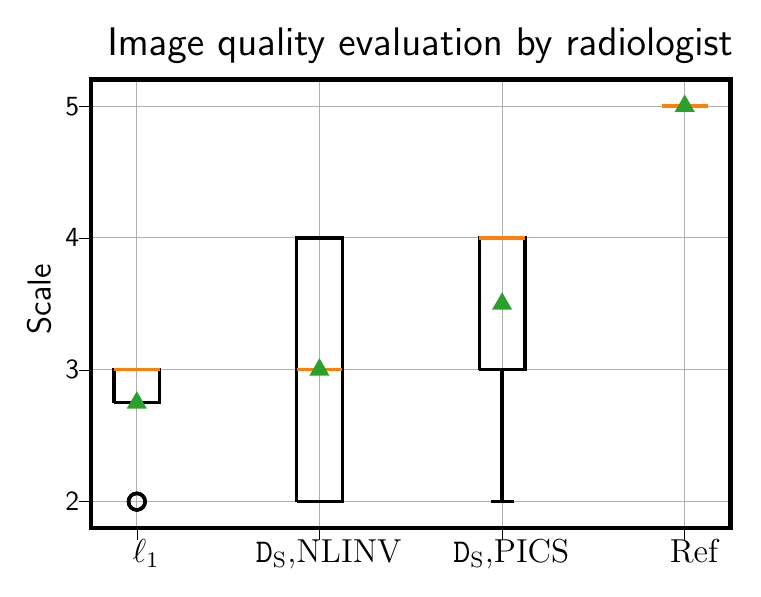
\begin{tikzpicture}
    \def\axisdefaultwidth{0.8\textwidth}
    \def\axisdefaultheight{0.6\textwidth}
\definecolor{darkgray176}{RGB}{176,176,176}
\definecolor{darkorange25512714}{RGB}{255,127,14}
\definecolor{forestgreen4416044}{RGB}{44,160,44}

\begin{axis}[
tick align=outside,
tick pos=left,
title={Image quality evaluation by radiologist },
x grid style={darkgray176},
xmajorgrids,
xmin=-0.5, xmax=6.5,
xtick style={color=black},
xtick={0,2,4,6},
xticklabels={$\ell_1$, \texttt{D}\textsubscript{S}{,}NLINV, \texttt{D}\textsubscript{S}{,}PICS, Ref},
y grid style={darkgray176},
ylabel={Scale},
ymajorgrids,
ymin=1.8, ymax=5.2,
ytick style={color=black}
]
\addplot [black]
table {%
-0.25 2.75
0.25 2.75
0.25 3
-0.25 3
-0.25 2.75
};
\addplot [black]
table {%
0 2.75
0 2.75
};
\addplot [black]
table {%
0 3
0 3
};
\addplot [black]
table {%
-0.125 2.75
0.125 2.75
};
\addplot [black]
table {%
-0.125 3
0.125 3
};
\addplot [black, mark=o, mark size=3, mark options={solid,fill opacity=0}, only marks]
table {%
0 2
0 2
0 2
};
\addplot [black]
table {%
1.75 2
2.25 2
2.25 4
1.75 4
1.75 2
};
\addplot [black]
table {%
2 2
2 2
};
\addplot [black]
table {%
2 4
2 4
};
\addplot [black]
table {%
1.875 2
2.125 2
};
\addplot [black]
table {%
1.875 4
2.125 4
};
\addplot [black]
table {%
3.75 3
4.25 3
4.25 4
3.75 4
3.75 3
};
\addplot [black]
table {%
4 3
4 2
};
\addplot [black]
table {%
4 4
4 4
};
\addplot [black]
table {%
3.875 2
4.125 2
};
\addplot [black]
table {%
3.875 4
4.125 4
};
\addplot [black]
table {%
5.75 5
6.25 5
6.25 5
5.75 5
5.75 5
};
\addplot [black]
table {%
6 5
6 5
};
\addplot [black]
table {%
6 5
6 5
};
\addplot [black]
table {%
5.875 5
6.125 5
};
\addplot [black]
table {%
5.875 5
6.125 5
};
\addplot [darkorange25512714]
table {%
-0.25 3
0.25 3
};
\addplot [forestgreen4416044, mark=triangle*, mark size=3, mark options={solid}, only marks]
table {%
0 2.75
};
\addplot [darkorange25512714]
table {%
1.75 3
2.25 3
};
\addplot [forestgreen4416044, mark=triangle*, mark size=3, mark options={solid}, only marks]
table {%
2 3
};
\addplot [darkorange25512714]
table {%
3.75 4
4.25 4
};
\addplot [forestgreen4416044, mark=triangle*, mark size=3, mark options={solid}, only marks]
table {%
4 3.5
};
\addplot [darkorange25512714]
table {%
5.75 5
6.25 5
};
\addplot [forestgreen4416044, mark=triangle*, mark size=3, mark options={solid}, only marks]
table {%
6 5
};
\end{axis}

\end{tikzpicture}

}
\end{mdframed}

\end{document}
